\documentclass{beamer}
\usepackage{etex} % to avoid errors http://tex.stackexchange.com/questions/7896/no-room-for-a-new-dimen-when-including-tikz
\usepackage{ulem}
\usepackage{listings}
\usepackage{slashbox}
\usepackage{tikz}
\usepackage[all]{xy}
\usepackage{booktabs}
\usepackage{amsmath,amssymb}
\usepackage{hyperref}
\usepackage{graphicx}

\DeclareMathOperator*{\argmin}{arg\,min}
\DeclareMathOperator*{\argmax}{arg\,max}
\DeclareMathOperator*{\maximize}{maximize}
\DeclareMathOperator*{\minimize}{minimize}
\newcommand{\sign}{\operatorname{sign}}
\newcommand{\RR}{\mathbb R}
\newcommand{\NN}{\mathbb N}

% Set transparency of non-highlighted sections in the table of
% contents slide.
\setbeamertemplate{section in toc shaded}[default][100]
\AtBeginSection[]
{
  \setbeamercolor{section in toc}{fg=red} 
  \setbeamercolor{section in toc shaded}{fg=black} 
  \begin{frame}
    \tableofcontents[currentsection]
  \end{frame}
}

\begin{document}

\title{Supervised, interactive genomic data analysis}
\author{
Toby Dylan Hocking
}

\date{Barbados workshop, 5--9 January 2015}

\maketitle

\section{Some problems with unsupervised
  DNA copy number analysis}

\begin{frame}
  \frametitle{DNA copy number analysis}

  Figure source: Alberts \textit{et al.} 2002. Molecular Biology of the Cell.
\vskip 0.1in
  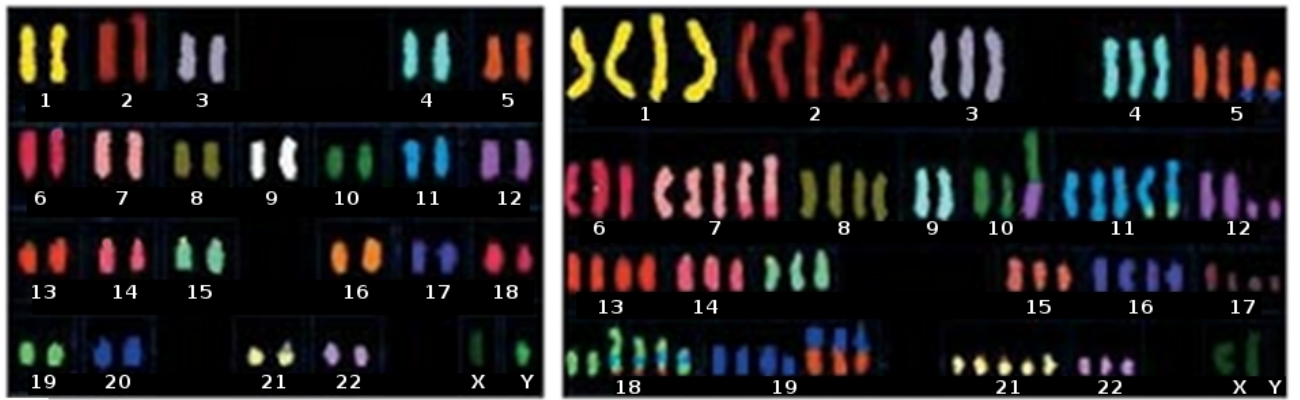
\includegraphics[width=\textwidth]{Karyo-both}
\vskip 0.1in
  \begin{minipage}{0.4\linewidth}
    Normal cell with 2 copies of each autosome.
  \end{minipage}
\hskip 0.1\linewidth
  \begin{minipage}{0.4\linewidth}
Cancer cell with many copy number alterations.
  \end{minipage}

\end{frame}

\begin{frame}
  \frametitle{Unsupervised, non-interactive DNA copy number analysis}
  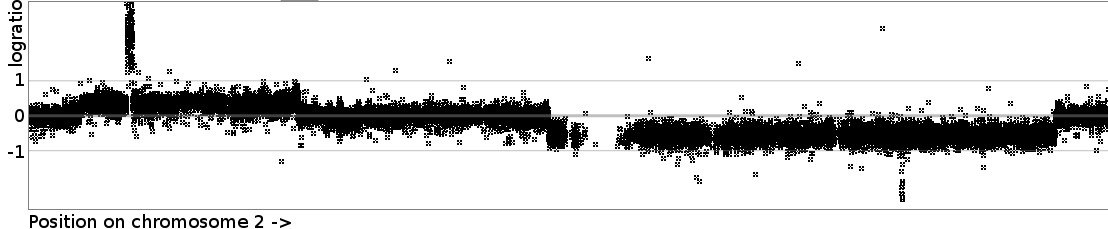
\includegraphics[width=\textwidth]{unlabeled-axes}

  Analyst sees a vector of $d$ noisy data points $\mathbf x\in\RR^d$.

  \vskip 0.1in

  \textbf{Question:}\\
  where are the true changes in copy
  number? (breakpoints)

\end{frame}

\begin{frame}
  \frametitle{Unsupervised, non-interactive DNA copy number analysis}

  \textbf{Unsupervised default model:} 
  fit a breakpoint model $f(\mathbf x, \lambda)$.\\
  ($\lambda$ is a model parameter, for example a p-value threshold or
  the number of breakpoints)

  \begin{displaymath}
  \xymatrix{
    \text{Data $\mathbf x$}
    \ar `[r] [dr] 
    & \text{ }
    \\
    % \text{Plot} \ar@{->}[d]
    & 
    \text{Model $f(\mathbf x, \lambda)$} 
    \\
    % \text{Labels $\mathbf y$}       \ar@{->}[d]
    \\
    \text{Parameter $\lambda$} 
    \ar `r[ruu] [ruu]
    & \text{ }
  }
  \end{displaymath}
  
  \textbf{Problem}: how do we know the model $f$ and parameter
  $\lambda$ are reasonable?

  \vskip 0.1in

  \textbf{Solution:} plot breakpoints $f(\mathbf x, \lambda)$ and
  interactively choose a reasonable parameter $\lambda$.
\end{frame}

\begin{frame}
  \frametitle{Unsupervised, interactive DNA copy number analysis}
  Analyst sees a vector of $d$ noisy data points $\mathbf x\in\RR^d$, \\
  and the model breakpoints $f(\mathbf x, \lambda)$.

  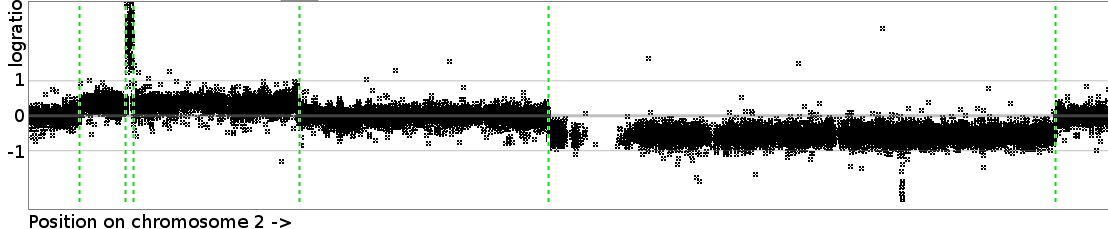
\includegraphics[width=\textwidth]{unlabeled-breakpoints-6}

  Parameter $\lambda$ = 6 breakpoints.
\end{frame}

\begin{frame}
  \frametitle{Unsupervised, interactive DNA copy number analysis}
  Analyst sees a vector of $d$ noisy data points $\mathbf x\in\RR^d$, \\
  and the model breakpoints $f(\mathbf x, \lambda)$.

  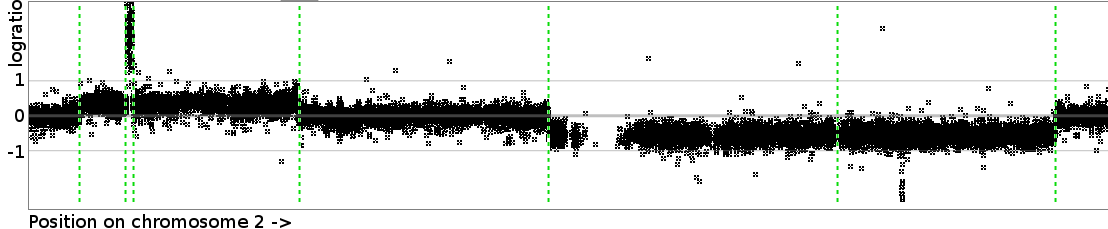
\includegraphics[width=\textwidth]{unlabeled-breakpoints-7}

  Parameter $\lambda$ = 7 breakpoints.
\end{frame}

\begin{frame}
  \frametitle{Unsupervised, interactive DNA copy number analysis}
  Analyst sees a vector of $d$ noisy data points $\mathbf x\in\RR^d$, \\
  and the model breakpoints $f(\mathbf x, \lambda)$.

  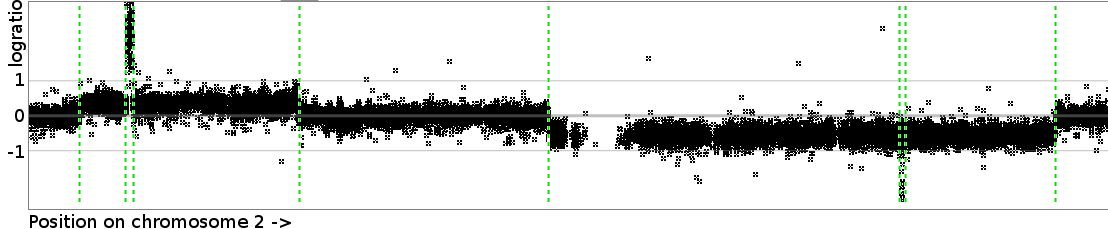
\includegraphics[width=\textwidth]{unlabeled-breakpoints-8}

  Parameter $\lambda$ = 8 breakpoints.
\end{frame}

\begin{frame}
  \frametitle{Unsupervised, interactive DNA copy number analysis}
  Analyst sees a vector of $d$ noisy data points $\mathbf x\in\RR^d$, \\
  and the model breakpoints $f(\mathbf x, \lambda)$.

  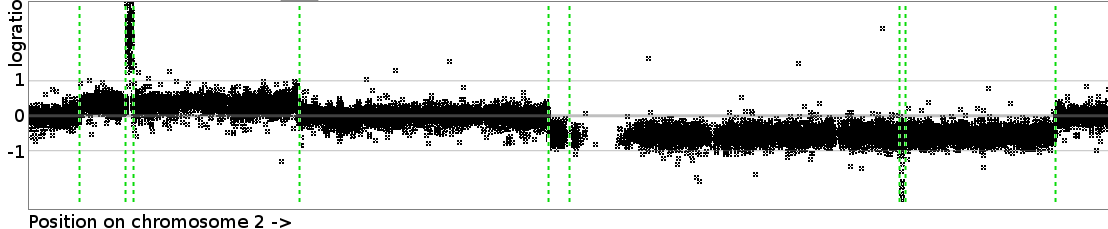
\includegraphics[width=\textwidth]{unlabeled-breakpoints-9}

  Parameter $\lambda$ = 9 breakpoints.
\end{frame}

\begin{frame}
  \frametitle{A brief history of unsupervised DNA copy number analysis}
  \begin{itemize}
  \item GLAD: adaptive weights smoothing (Hup\'e \textit{et al.}, 2004)
  \item DNAcopy: circular binary segmentation (Venkatraman and Olshen,
    2007)
  \item cghFLasso: fused lasso signal approximator with heuristics
    (Tibshirani and Wang, 2007)
  \item HaarSeg: wavelet smoothing (Ben-Yaacov and Eldar, 2008)
  \item GADA: sparse Bayesian learning (Pique-Regi \textit{et al.}, 2008)
  \item flsa: fused lasso signal approximator path algorithm (Hoefling 2009)
  \item cghseg: pruned dynamic programming (Rigaill 2010)
  \item PELT: pruned exact linear time (Killick \textit{et al.}, 2011)
  \end{itemize}
  Demo: \url{http://compbio.med.harvard.edu/CGHweb/}
\end{frame}

\begin{frame}
  \frametitle{Unsupervised, interactive DNA copy number analysis}
  
  Non-interactive unsupervised default model.
  
  \small

  \begin{displaymath}
  \xymatrix{
    \text{Data $\mathbf x$}
    \ar `[r] [dr] 
    %\ar `r[rr] [drr] 
    %\ar `r[rrr] [drrr] 
    %\ar [d]
    & \text{ }
    & \text{ }
    & \text{ }
    \\
    %\text{Plot} 
    %\ar [d]
    & 
    \text{Model $f(\mathbf x, \lambda_1)$} 
    %\ar [r]
    & 
    \textcolor{white}{\text{Plot}}
    %\ar[dd]
    &
    \color{white}{ \text{Model $f(\mathbf x, \lambda_2)$} }
    \\
    %\text{Labels $\mathbf y$}       
    %\ar [d]
    & 
    &
    \\
    \text{Parameter $\lambda_1$} 
    \ar `r[ruu] [ruu]
    %\ar [rr]
    & \text{ }
    & \color{white}{ \text{Parameter $\lambda_2$} }
    %\ar `r[ruu] [ruu] 
  }
  \end{displaymath}
\end{frame}

\begin{frame}
  \frametitle{Unsupervised, interactive DNA copy number analysis}

  Plot the default model.
  
  \small

  \begin{displaymath}
  \xymatrix{
    \text{Data $\mathbf x$}
    \ar `[r] [dr] 
    \ar `r[rr] [drr] 
    %\ar `r[rrr] [drrr] 
    %\ar [d]
    & \text{ }
    & \text{ }
    & \text{ }
    \\
    %\text{Plot} 
    %\ar [d]
    & 
    \text{Model $f(\mathbf x, \lambda_1)$} 
    \ar [r]
    & 
    \text{Plot}
    %\ar[dd]
    &
    \color{white}{ \text{Model $f(\mathbf x, \lambda_2)$} }
    \\
    %\text{Labels $\mathbf y$}       
    %\ar [d]
    & 
    &
    \\
    \text{Parameter $\lambda_1$} 
    \ar `r[ruu] [ruu]
    %\ar [rr]
    & \text{ }
    & \color{white}{ \text{Parameter $\lambda_2$} }
    %\ar `r[ruu] [ruu] 
  }
  \end{displaymath}
\end{frame}

\begin{frame}
  \frametitle{Unsupervised, interactive DNA copy number analysis}

  Increase/decrease parameter based on signal/noise in plot.
  
  \small

  \begin{displaymath}
  \xymatrix{
    \text{Data $\mathbf x$}
    \ar `[r] [dr] 
    \ar `r[rr] [drr] 
    %\ar `r[rrr] [drrr] 
    %\ar [d]
    & \text{ }
    & \text{ }
    & \text{ }
    \\
    %\text{Plot} 
    %\ar [d]
    & 
    \text{Model $f(\mathbf x, \lambda_1)$} 
    \ar [r]
    & 
    \text{Plot}
    \ar[dd]
    &
    \color{white}{ \text{Model $f(\mathbf x, \lambda_2)$} }
    \\
    %\text{Labels $\mathbf y$}       
    %\ar [d]
    & 
    &
    \\
    \text{Parameter $\lambda_1$} 
    \ar `r[ruu] [ruu]
    \ar [rr]
    & \text{ }
    & \text{Parameter $\lambda_2$}
    %\ar `r[ruu] [ruu] 
  }
  \end{displaymath}
\end{frame}

\begin{frame}
  \frametitle{Unsupervised, interactive DNA copy number analysis}

  Fit model using new parameter.
  
  \small

  \begin{displaymath}
  \xymatrix{
    \text{Data $\mathbf x$}
    \ar `[r] [dr] 
    \ar `r[rr] [drr] 
    \ar `r[rrr] [drrr] 
    %\ar [d]
    & \text{ }
    & \text{ }
    & \text{ }
    \\
    %\text{Plot} 
    %\ar [d]
    & 
    \text{Model $f(\mathbf x, \lambda_1)$} 
    \ar [r]
    & 
    \text{Plot}
    \ar[dd]
    &
    \text{Model $f(\mathbf x, \lambda_2)$} 
    \\
    %\text{Labels $\mathbf y$}       
    %\ar [d]
    & 
    &
    \\
    \text{Parameter $\lambda_1$} 
    \ar `r[ruu] [ruu]
    \ar [rr]
    & \text{ }
    & \text{Parameter $\lambda_2$}
    \ar `r[ruu] [ruu] 
  }
  \end{displaymath}
\end{frame}

\begin{frame}
  \frametitle{Summary of unsupervised models, software}

  \begin{center}
  \begin{tabular}{c|c|c}
    Evaluation: & qualitative &  \\
    Input: profile $\mathbf x$ + & parameters $\lambda$ &  \\
        & \textbf{unsupervised} & \\
    \hline
    \textbf{non-interactive}
    & plot $\mathbf x$\\
    fit one model 
    & default parameters &  \\
    & e.g. DNAcopy \\
    \hline
    \textbf{interactive}
    & plot $\mathbf x, f(\mathbf x, \lambda)$\\
    plot, update model 
    & tuned parameters & \\
    & e.g. CGHweb  
  \end{tabular}
  \end{center}

  Works fine for 1 profile, but...

\end{frame}

\begin{frame}
  \frametitle{Unsupervised, interactive DNA copy number analysis\\
  with 3 profiles (in practice we have 1000s)}
  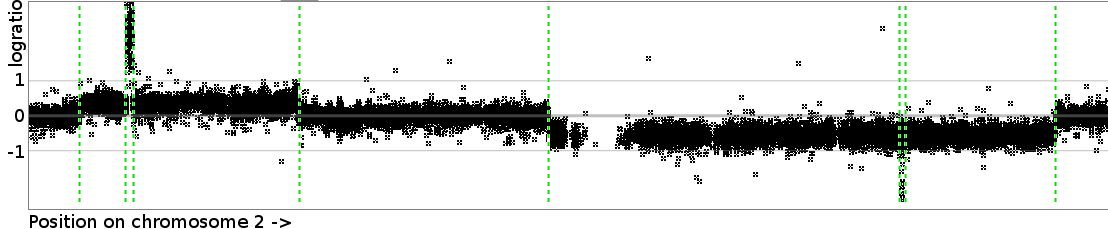
\includegraphics[width=\textwidth]{unlabeled-breakpoints-8}

  Parameter $\lambda_1$ = 8 breakpoints.

  \vskip 0.1in

  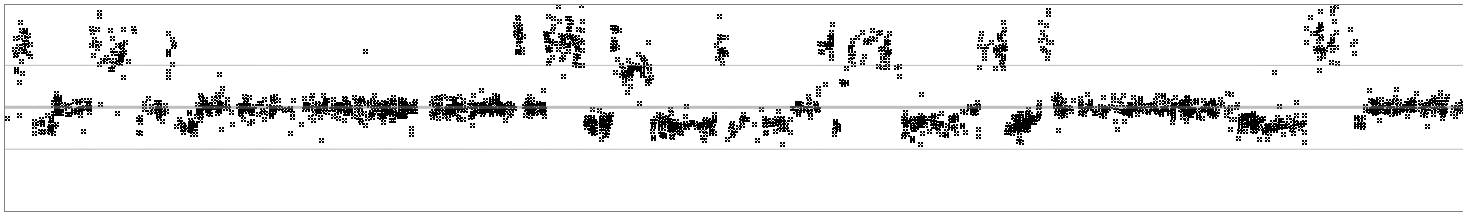
\includegraphics[width=\textwidth]{lots-of-breaks}

  Parameter $\lambda_2$ = ??

  \vskip 0.1in

  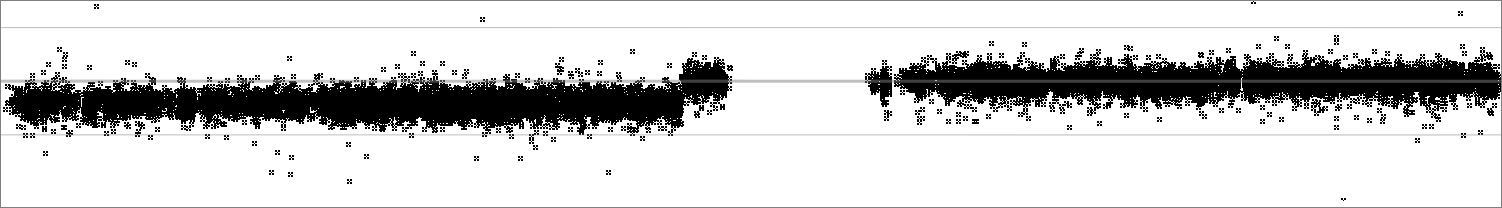
\includegraphics[width=\textwidth]{only-one-break}

  Parameter $\lambda_3$ = ??

\end{frame}

\begin{frame}
  \frametitle{Some problems with unsupervised analysis}
  \textbf{Training a model that works on many samples and genomic
    regions?} 
  \begin{itemize}
  \item What if we don't have time to look at all samples/regions and
      interactively select a good parameter $\lambda$ for each?
  % \item \textbf{Generalization:} how does the parameter for one
  %   profile $\lambda_1$ help us choose a parameter $\lambda_2, \lambda_3$
  %   for other profiles?
  % \item \textbf{What if we use a different model $g(\mathbf x, \rho)$ where
  %   the learned $\lambda$ is meaningless?
  \item Use default parameter $\lambda$ for all profiles?
  \item If we know a good parameter $\lambda_1=8$ for one profile, 
    does that help us choose a parameter $\lambda_2, \lambda_3$ for
    other profiles?
  \item How does knowledge that $\lambda_1=8$ is good help us train
    another model $g(\mathbf x, \rho)$ with a different parameter
    $\rho$?
  \end{itemize}
  \textbf{Testing different models of the same data?} 
    \begin{itemize}
    \item   Are the breakpoints of $f(\mathbf x, \lambda$) or
  $g(\mathbf x, \rho)$ better?
    \item Plot the data and both models, qualitative visual evaluation?
    \end{itemize}
  All of these problems can be solved by supervised learning.
\end{frame}

\section{Supervised DNA copy number analysis}

\begin{frame}
  \frametitle{Computer vision: look and add labels to...}
  \begin{tabular}{ccc}
    Photos & Cell images & Copy number profiles \\
    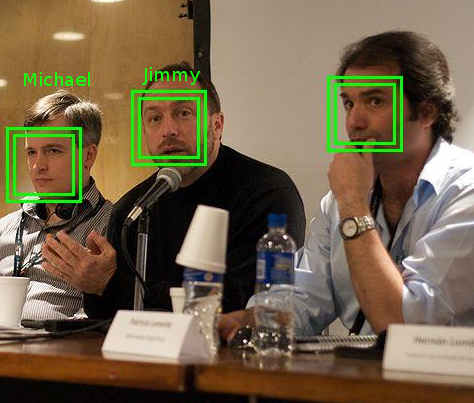
\includegraphics[width=1.3in]{faces} &
    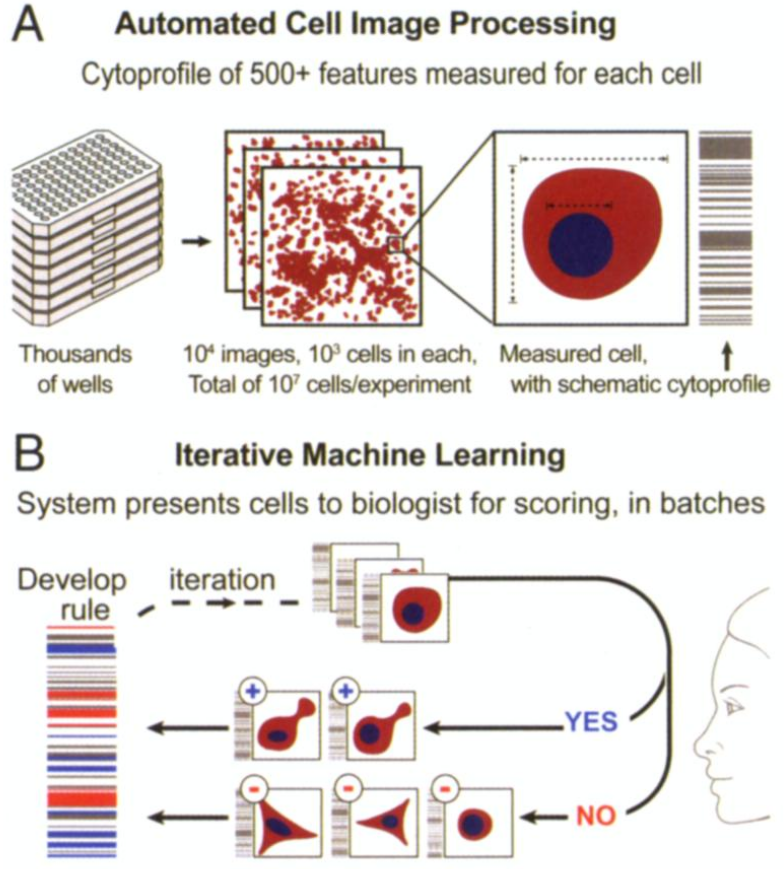
\includegraphics[width=1.3in]{cellprofiler} &
    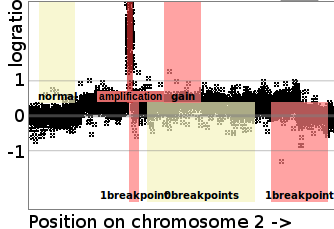
\includegraphics[width=1.5in]{regions-axes}\\
    Labels: faces, names & phenotypes & alterations \\
    CVPR 2013 & CellProfiler & SegAnnDB \\
    246 papers & 873 citations & H, \textit{et al.} 2014. \\
     &
  \end{tabular}
  Sources: \url{http://en.wikipedia.org/wiki/Face_detection}\\
  Jones et al PNAS 2009. Scoring diverse cellular morphologies in
  image-based screens with iterative feedback and machine learning.
\end{frame}

\begin{frame}
  \frametitle{Computer vision for genomic segmentation}
  \begin{center}
  \begin{tabular}{rll}
    \textbf{Breakpoint}\\
 \textbf{detector} & \textbf{strong point} & \textbf{weak point} \\
    \hline
    mathematical  & maximum likelihood & tuning parameters $\lambda$ \\
    models & algorithm finds exact  & chosen using\\
& breakpoint locations  & unrealistic assumptions\\
    \hline
    your eyes & outliers, signal/noise & finding the \\
    & over large regions &  exact breakpoint
  \end{tabular}
  \end{center}
  % \vskip 1cm
  % \textbf{SegAnnDB exploits the strong points of both:}
  % \begin{itemize}
  % \item Plot a maximum likelihood model alongside the data.
  % \item Edit annotated regions.
  % \item The model parameters are automatically updated to agree.
  % \item No tuning parameters, but need to annotate a few profiles.
  % \end{itemize}
  % Demo on \url{http://bioviz.rocq.inria.fr/}

  Discussion of common objections:
  \begin{itemize}
  \item \textbf{Isn't this totally subjective?} Yes, guilty as
    charged. \\
    But so is everything else we do, including choice of
    model $f$ and parameter $\lambda$.
  \item \textbf{Won't the results change based on the annotator?}
    Possibly, but usually annotators agree.
  \end{itemize}
\end{frame}

\begin{frame}[fragile]
  \frametitle{Supervised, non-interactive DNA copy number analysis}

  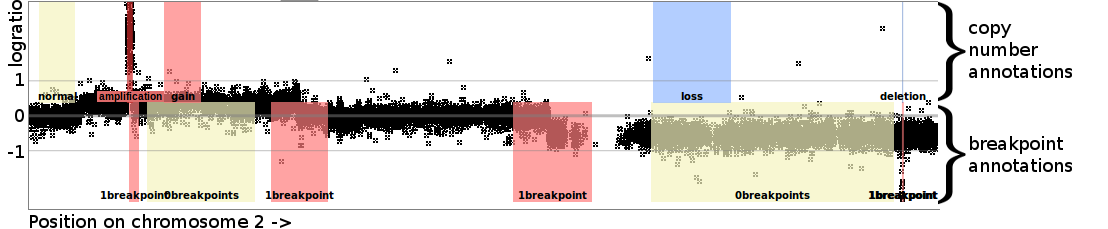
\includegraphics[width=\textwidth]{regions-axes-full}

  Analyst sees a vector of $d$ noisy data points $\mathbf x\in\RR^d$,\\
  and some manually annotated region labels $\mathbf y$.

  \vskip 0.1in

  \textbf{Question:}\\
    where are the true changes in copy number? (breakpoints)

  \vskip 0.1in

  But wait!

  \vskip 0.1in
  
  I learned in my Statistics 101 class that ``all models are wrong,
  but some are useful.''

\end{frame}

\begin{frame}[fragile]
  \frametitle{Aside: George Box (1919--2013)}
  \small \url{http://www-history.mcs.st-and.ac.uk/Biographies/Box.html}
  \begin{description}
  \item[1919] Born in England, wanted to study chemistry.
  \item[1942] Drafted in WW2, ended up doing statistics.
  \item[1945] Married Jessie Ward.
  \item[1953] PhD advised by Egon Pearson at UCL.
  \item[1959] Married Joan G Fisher. (Ronald Fisher's second daughter)
  \item[1960] Founded Statistics Department at University of Wisconsin.
  \item[1964] Box and Cox, An analysis of transformations (JRSSB).
  \item[1985] Married Claire Louise Quist.
  \item[1987] Box and Draper, \textit{Empirical model-building and
      response surfaces}, page 424:
  \end{description}

  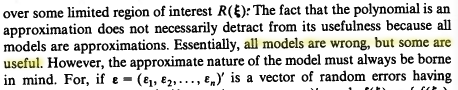
\includegraphics[width=0.8\textwidth]{Box-Draper-all-models-are-wrong-but-some-are-useful-hilite}

  Not the inventor of the box plot! (that was John Tukey, 1970)

\end{frame}

\begin{frame}[fragile]
  \frametitle{Supervised, non-interactive DNA copy number analysis}

  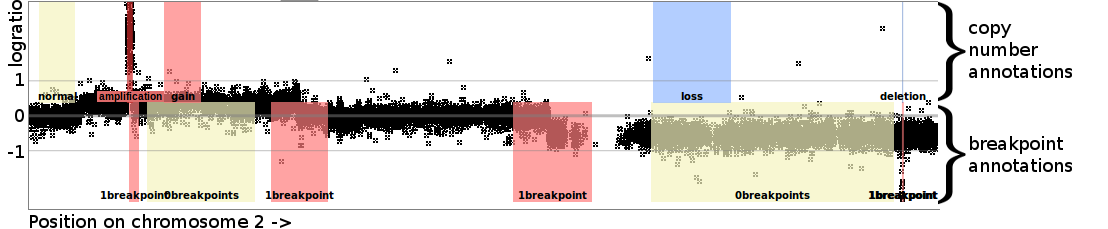
\includegraphics[width=\textwidth]{regions-axes-full}

  Analyst sees a vector of $d$ noisy data points $\mathbf x\in\RR^d$,\\
  and some manually annotated region labels $\mathbf y$.

  \vskip 0.1in

  \sout{\textbf{Question:}\\
    where are the true changes in copy number? (breakpoints)}

  \vskip 0.1in

  ``Essentially, all models are wrong, but some are useful.''\\
  Box and Draper (1987).

  \vskip 0.5cm

  \textbf{Train question:} can we fit a model $f(\mathbf x, \lambda)$
  to the labels $\mathbf y?$
  \\
  \textbf{Test question:} does the fitted model $f(\mathbf x^*, \lambda)$
  have good predictions for test data $\mathbf x^*$ and labels $\mathbf y^*$?

\end{frame}

\begin{frame}
  \frametitle{Supervised training of breakpoint detection model}

  Reference: Hocking \textit{et al.} Learning smoothing models of copy
  number profiles using breakpoint annotations, BMC Bioinfo
  (2013).

  \begin{center}
      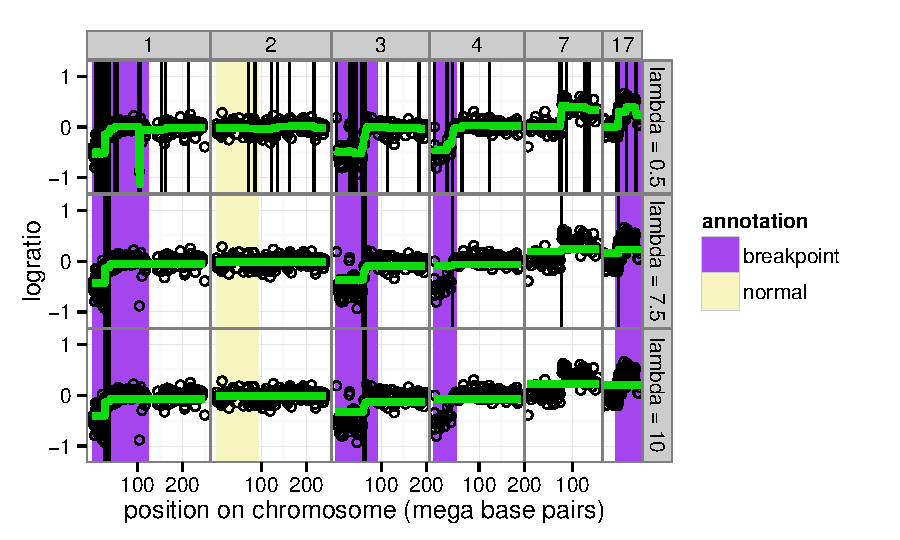
\includegraphics[width=0.7\textwidth]{bams-smoothing}
  \end{center}

  Find the best parameter $\lambda$ for $n=6$ profiles $\mathbf x_i$
  with labels $\mathbf y_i$:

  \begin{equation*}
    \hat \lambda = \argmin_{\lambda}
    \sum_{i=1}^n
    E\big[
      \mathbf y_i,
      f(\mathbf x_i, \lambda)
    \big].
  \end{equation*}

  $E$ is zero-one loss (number of incorrect regions).

\end{frame}


\begin{frame}
  \frametitle{Ranking breakpoint detectors by test error}

  Benchmark data set, R package \texttt{neuroblastoma}:
  profiles~$\mathbf x_i$ from 575 neuroblastoma patients, two
  different sets of labels $\mathbf y_i$:
  \begin{description}
  \item[Original] 3418 manually annotated regions (type 0/1 in Excel).
  \item[Detailed] 4359 manually annotated regions (custom GUI).
  \end{description}

  \begin{center}
    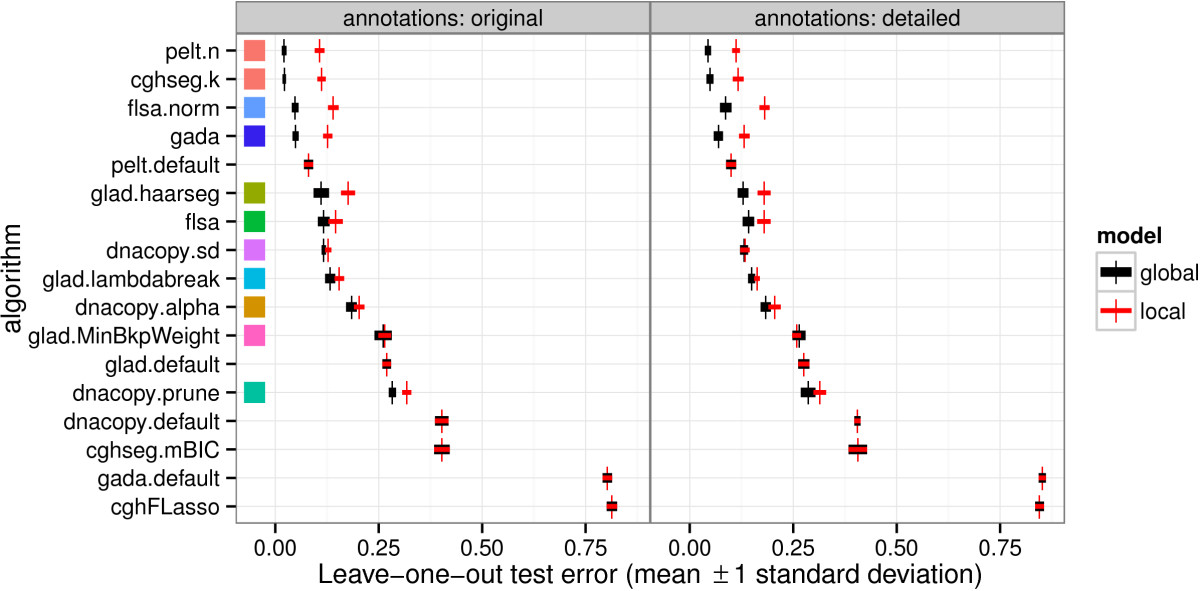
\includegraphics[width=0.8\textwidth]{bams-test-error}
  \end{center}

  \begin{description}
  \item[Local model] choose best scalar $\lambda_i$ for each profile $i$.\\
  \item[Global model] choose best scalar $\lambda$ overall.
  \end{description}
\end{frame}

\begin{frame}
  \frametitle{Learning a multi-parameter penalty function}
  \begin{center}
    % Created by tikzDevice version 0.7.0 on 2014-12-22 10:27:21
% !TEX encoding = UTF-8 Unicode
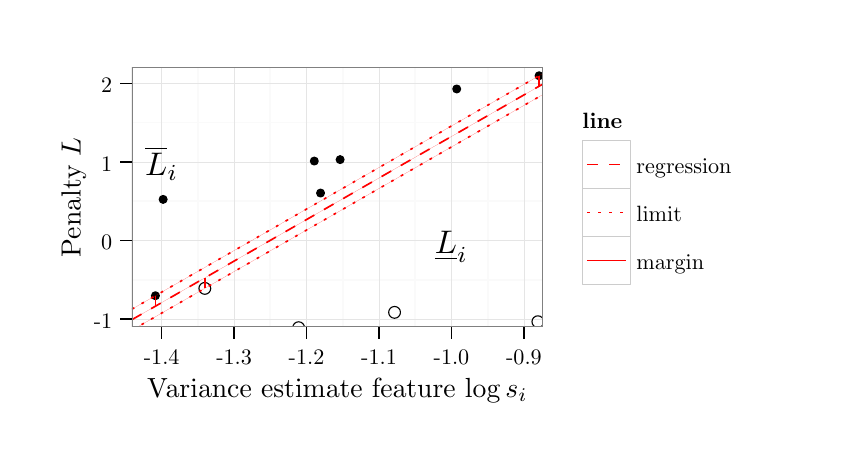
\begin{tikzpicture}[x=1pt,y=1pt]
\definecolor[named]{fillColor}{rgb}{1.00,1.00,1.00}
\path[use as bounding box,fill=fillColor,fill opacity=0.00] (0,0) rectangle (289.08,144.54);
\begin{scope}
\path[clip] (  0.00,  0.00) rectangle (289.08,144.54);
\definecolor[named]{drawColor}{rgb}{1.00,1.00,1.00}
\definecolor[named]{fillColor}{rgb}{1.00,1.00,1.00}

\path[draw=drawColor,line width= 0.6pt,line join=round,line cap=round,fill=fillColor] (  0.00,  0.00) rectangle (289.08,144.54);
\end{scope}
\begin{scope}
\path[clip] ( 37.66, 36.44) rectangle (186.13,130.09);
\definecolor[named]{fillColor}{rgb}{1.00,1.00,1.00}

\path[fill=fillColor] ( 37.66, 36.44) rectangle (186.13,130.09);
\definecolor[named]{drawColor}{rgb}{0.98,0.98,0.98}

\path[draw=drawColor,line width= 0.6pt,line join=round] ( 37.66, 53.47) --
	(186.13, 53.47);

\path[draw=drawColor,line width= 0.6pt,line join=round] ( 37.66, 81.85) --
	(186.13, 81.85);

\path[draw=drawColor,line width= 0.6pt,line join=round] ( 37.66,110.22) --
	(186.13,110.22);

\path[draw=drawColor,line width= 0.6pt,line join=round] ( 61.50, 36.44) --
	( 61.50,130.09);

\path[draw=drawColor,line width= 0.6pt,line join=round] ( 87.68, 36.44) --
	( 87.68,130.09);

\path[draw=drawColor,line width= 0.6pt,line join=round] (113.87, 36.44) --
	(113.87,130.09);

\path[draw=drawColor,line width= 0.6pt,line join=round] (140.05, 36.44) --
	(140.05,130.09);

\path[draw=drawColor,line width= 0.6pt,line join=round] (166.23, 36.44) --
	(166.23,130.09);
\definecolor[named]{drawColor}{rgb}{0.90,0.90,0.90}

\path[draw=drawColor,line width= 0.2pt,line join=round] ( 37.66, 39.28) --
	(186.13, 39.28);

\path[draw=drawColor,line width= 0.2pt,line join=round] ( 37.66, 67.66) --
	(186.13, 67.66);

\path[draw=drawColor,line width= 0.2pt,line join=round] ( 37.66, 96.03) --
	(186.13, 96.03);

\path[draw=drawColor,line width= 0.2pt,line join=round] ( 37.66,124.41) --
	(186.13,124.41);

\path[draw=drawColor,line width= 0.2pt,line join=round] ( 48.41, 36.44) --
	( 48.41,130.09);

\path[draw=drawColor,line width= 0.2pt,line join=round] ( 74.59, 36.44) --
	( 74.59,130.09);

\path[draw=drawColor,line width= 0.2pt,line join=round] (100.78, 36.44) --
	(100.78,130.09);

\path[draw=drawColor,line width= 0.2pt,line join=round] (126.96, 36.44) --
	(126.96,130.09);

\path[draw=drawColor,line width= 0.2pt,line join=round] (153.14, 36.44) --
	(153.14,130.09);

\path[draw=drawColor,line width= 0.2pt,line join=round] (179.32, 36.44) --
	(179.32,130.09);
\definecolor[named]{drawColor}{rgb}{0.00,0.00,0.00}

\node[text=drawColor,anchor=base,inner sep=0pt, outer sep=0pt, scale=  1.18] at (153.14, 62.78) {$\underline L_i$};

\node[text=drawColor,anchor=base,inner sep=0pt, outer sep=0pt, scale=  1.18] at ( 48.41, 91.15) {$\overline L_i$};

\path[draw=drawColor,line width= 0.4pt,line join=round,line cap=round] ( 64.01, 50.33) circle (  2.13);

\path[draw=drawColor,line width= 0.4pt,line join=round,line cap=round] (184.36, 38.29) circle (  2.13);

\path[draw=drawColor,line width= 0.4pt,line join=round,line cap=round] (153.38,  6.61) circle (  2.13);

\path[draw=drawColor,line width= 0.4pt,line join=round,line cap=round] (186.13, 24.56) circle (  2.13);

\path[draw=drawColor,line width= 0.4pt,line join=round,line cap=round] (132.57, 41.67) circle (  2.13);

\path[draw=drawColor,line width= 0.4pt,line join=round,line cap=round] ( 94.46, 29.21) circle (  2.13);

\path[draw=drawColor,line width= 0.4pt,line join=round,line cap=round] (112.83, 16.84) circle (  2.13);

\path[draw=drawColor,line width= 0.4pt,line join=round,line cap=round] (118.78, 11.51) circle (  2.13);

\path[draw=drawColor,line width= 0.4pt,line join=round,line cap=round] (120.11, 23.68) circle (  2.13);

\path[draw=drawColor,line width= 0.4pt,line join=round,line cap=round] (114.20, 21.12) circle (  2.13);

\path[draw=drawColor,line width= 0.4pt,line join=round,line cap=round] (141.34,  4.11) circle (  2.13);

\path[draw=drawColor,line width= 0.4pt,line join=round,line cap=round] (121.45, -0.45) circle (  2.13);

\path[draw=drawColor,line width= 0.4pt,line join=round,line cap=round] (148.35, -0.62) circle (  2.13);

\path[draw=drawColor,line width= 0.4pt,line join=round,line cap=round] ( 97.91, 36.13) circle (  2.13);

\path[draw=drawColor,line width= 0.4pt,line join=round,line cap=round] (104.19, 30.95) circle (  2.13);

\path[draw=drawColor,line width= 0.4pt,line join=round,line cap=round] ( 79.92, 15.58) circle (  2.13);
\definecolor[named]{fillColor}{rgb}{0.00,0.00,0.00}

\path[draw=drawColor,line width= 0.4pt,line join=round,line cap=round,fill=fillColor] ( 46.16, 47.68) circle (  1.42);

\path[draw=drawColor,line width= 0.4pt,line join=round,line cap=round,fill=fillColor] (112.90, 96.86) circle (  1.42);

\path[draw=drawColor,line width= 0.4pt,line join=round,line cap=round,fill=fillColor] ( 48.95, 82.49) circle (  1.42);

\path[draw=drawColor,line width= 0.4pt,line join=round,line cap=round,fill=fillColor] (184.80,127.17) circle (  1.42);

\path[draw=drawColor,line width= 0.4pt,line join=round,line cap=round,fill=fillColor] (105.83, 84.78) circle (  1.42);

\path[draw=drawColor,line width= 0.4pt,line join=round,line cap=round,fill=fillColor] (103.57, 96.34) circle (  1.42);

\path[draw=drawColor,line width= 0.4pt,line join=round,line cap=round,fill=fillColor] (155.03,122.39) circle (  1.42);
\definecolor[named]{drawColor}{rgb}{1.00,0.00,0.00}
\definecolor[named]{fillColor}{rgb}{1.00,0.00,0.00}

\path[draw=drawColor,line width= 0.6pt,dash pattern=on 4pt off 4pt ,line join=round,fill=fillColor] ( 37.66, 39.02) -- (186.13,124.14);

\path[draw=drawColor,line width= 0.6pt,dash pattern=on 1pt off 3pt ,line join=round,fill=fillColor] ( 37.66, 42.81) -- (186.13,127.93);

\path[draw=drawColor,line width= 0.6pt,dash pattern=on 1pt off 3pt ,line join=round,fill=fillColor] ( 37.66, 35.23) -- (186.13,120.35);

\path[draw=drawColor,line width= 0.6pt,line join=round,fill=fillColor] ( 64.01, 50.33) -- ( 64.01, 54.12);

\path[draw=drawColor,line width= 0.6pt,line join=round,fill=fillColor] ( 46.16, 47.68) -- ( 46.16, 43.89);

\path[draw=drawColor,line width= 0.6pt,line join=round,fill=fillColor] (184.80,127.17) -- (184.80,123.38);
\definecolor[named]{drawColor}{rgb}{0.50,0.50,0.50}

\path[draw=drawColor,line width= 0.6pt,line join=round,line cap=round] ( 37.66, 36.44) rectangle (186.13,130.09);
\end{scope}
\begin{scope}
\path[clip] (  0.00,  0.00) rectangle (289.08,144.54);
\definecolor[named]{drawColor}{rgb}{0.00,0.00,0.00}

\node[text=drawColor,anchor=base east,inner sep=0pt, outer sep=0pt, scale=  0.80] at ( 30.55, 35.98) {-1};

\node[text=drawColor,anchor=base east,inner sep=0pt, outer sep=0pt, scale=  0.80] at ( 30.55, 64.35) {0};

\node[text=drawColor,anchor=base east,inner sep=0pt, outer sep=0pt, scale=  0.80] at ( 30.55, 92.73) {1};

\node[text=drawColor,anchor=base east,inner sep=0pt, outer sep=0pt, scale=  0.80] at ( 30.55,121.10) {2};
\end{scope}
\begin{scope}
\path[clip] (  0.00,  0.00) rectangle (289.08,144.54);
\definecolor[named]{drawColor}{rgb}{0.00,0.00,0.00}

\path[draw=drawColor,line width= 0.6pt,line join=round] ( 33.40, 39.28) --
	( 37.66, 39.28);

\path[draw=drawColor,line width= 0.6pt,line join=round] ( 33.40, 67.66) --
	( 37.66, 67.66);

\path[draw=drawColor,line width= 0.6pt,line join=round] ( 33.40, 96.03) --
	( 37.66, 96.03);

\path[draw=drawColor,line width= 0.6pt,line join=round] ( 33.40,124.41) --
	( 37.66,124.41);
\end{scope}
\begin{scope}
\path[clip] (  0.00,  0.00) rectangle (289.08,144.54);
\definecolor[named]{drawColor}{rgb}{0.00,0.00,0.00}

\path[draw=drawColor,line width= 0.6pt,line join=round] ( 48.41, 32.18) --
	( 48.41, 36.44);

\path[draw=drawColor,line width= 0.6pt,line join=round] ( 74.59, 32.18) --
	( 74.59, 36.44);

\path[draw=drawColor,line width= 0.6pt,line join=round] (100.78, 32.18) --
	(100.78, 36.44);

\path[draw=drawColor,line width= 0.6pt,line join=round] (126.96, 32.18) --
	(126.96, 36.44);

\path[draw=drawColor,line width= 0.6pt,line join=round] (153.14, 32.18) --
	(153.14, 36.44);

\path[draw=drawColor,line width= 0.6pt,line join=round] (179.32, 32.18) --
	(179.32, 36.44);
\end{scope}
\begin{scope}
\path[clip] (  0.00,  0.00) rectangle (289.08,144.54);
\definecolor[named]{drawColor}{rgb}{0.00,0.00,0.00}

\node[text=drawColor,anchor=base,inner sep=0pt, outer sep=0pt, scale=  0.80] at ( 48.41, 22.72) {-1.4};

\node[text=drawColor,anchor=base,inner sep=0pt, outer sep=0pt, scale=  0.80] at ( 74.59, 22.72) {-1.3};

\node[text=drawColor,anchor=base,inner sep=0pt, outer sep=0pt, scale=  0.80] at (100.78, 22.72) {-1.2};

\node[text=drawColor,anchor=base,inner sep=0pt, outer sep=0pt, scale=  0.80] at (126.96, 22.72) {-1.1};

\node[text=drawColor,anchor=base,inner sep=0pt, outer sep=0pt, scale=  0.80] at (153.14, 22.72) {-1.0};

\node[text=drawColor,anchor=base,inner sep=0pt, outer sep=0pt, scale=  0.80] at (179.32, 22.72) {-0.9};
\end{scope}
\begin{scope}
\path[clip] (  0.00,  0.00) rectangle (289.08,144.54);
\definecolor[named]{drawColor}{rgb}{0.00,0.00,0.00}

\node[text=drawColor,anchor=base,inner sep=0pt, outer sep=0pt, scale=  1.00] at (111.90, 10.84) {Variance estimate feature $\log s_i$};
\end{scope}
\begin{scope}
\path[clip] (  0.00,  0.00) rectangle (289.08,144.54);
\definecolor[named]{drawColor}{rgb}{0.00,0.00,0.00}

\node[text=drawColor,rotate= 90.00,anchor=base,inner sep=0pt, outer sep=0pt, scale=  1.00] at ( 19.11, 83.26) {Penalty $L$};
\end{scope}
\begin{scope}
\path[clip] (  0.00,  0.00) rectangle (289.08,144.54);
\definecolor[named]{fillColor}{rgb}{1.00,1.00,1.00}

\path[fill=fillColor] (196.20, 47.50) rectangle (264.55,119.03);
\end{scope}
\begin{scope}
\path[clip] (  0.00,  0.00) rectangle (289.08,144.54);
\definecolor[named]{drawColor}{rgb}{0.00,0.00,0.00}

\node[text=drawColor,anchor=base west,inner sep=0pt, outer sep=0pt, scale=  0.80] at (200.47,108.14) {\bfseries line};
\end{scope}
\begin{scope}
\path[clip] (  0.00,  0.00) rectangle (289.08,144.54);
\definecolor[named]{drawColor}{rgb}{0.80,0.80,0.80}
\definecolor[named]{fillColor}{rgb}{1.00,1.00,1.00}

\path[draw=drawColor,line width= 0.6pt,line join=round,line cap=round,fill=fillColor] (200.47, 86.46) rectangle (217.81,103.80);
\end{scope}
\begin{scope}
\path[clip] (  0.00,  0.00) rectangle (289.08,144.54);
\definecolor[named]{drawColor}{rgb}{1.00,0.00,0.00}

\path[draw=drawColor,line width= 0.6pt,dash pattern=on 4pt off 4pt ,line join=round] (202.20, 95.13) -- (216.08, 95.13);
\end{scope}
\begin{scope}
\path[clip] (  0.00,  0.00) rectangle (289.08,144.54);
\definecolor[named]{drawColor}{rgb}{0.80,0.80,0.80}
\definecolor[named]{fillColor}{rgb}{1.00,1.00,1.00}

\path[draw=drawColor,line width= 0.6pt,line join=round,line cap=round,fill=fillColor] (200.47, 69.11) rectangle (217.81, 86.46);
\end{scope}
\begin{scope}
\path[clip] (  0.00,  0.00) rectangle (289.08,144.54);
\definecolor[named]{drawColor}{rgb}{1.00,0.00,0.00}

\path[draw=drawColor,line width= 0.6pt,dash pattern=on 1pt off 3pt ,line join=round] (202.20, 77.78) -- (216.08, 77.78);
\end{scope}
\begin{scope}
\path[clip] (  0.00,  0.00) rectangle (289.08,144.54);
\definecolor[named]{drawColor}{rgb}{0.80,0.80,0.80}
\definecolor[named]{fillColor}{rgb}{1.00,1.00,1.00}

\path[draw=drawColor,line width= 0.6pt,line join=round,line cap=round,fill=fillColor] (200.47, 51.77) rectangle (217.81, 69.11);
\end{scope}
\begin{scope}
\path[clip] (  0.00,  0.00) rectangle (289.08,144.54);
\definecolor[named]{drawColor}{rgb}{1.00,0.00,0.00}

\path[draw=drawColor,line width= 0.6pt,line join=round] (202.20, 60.44) -- (216.08, 60.44);
\end{scope}
\begin{scope}
\path[clip] (  0.00,  0.00) rectangle (289.08,144.54);
\definecolor[named]{drawColor}{rgb}{0.00,0.00,0.00}

\node[text=drawColor,anchor=base west,inner sep=0pt, outer sep=0pt, scale=  0.80] at (219.98, 91.82) {regression};
\end{scope}
\begin{scope}
\path[clip] (  0.00,  0.00) rectangle (289.08,144.54);
\definecolor[named]{drawColor}{rgb}{0.00,0.00,0.00}

\node[text=drawColor,anchor=base west,inner sep=0pt, outer sep=0pt, scale=  0.80] at (219.98, 74.48) {limit};
\end{scope}
\begin{scope}
\path[clip] (  0.00,  0.00) rectangle (289.08,144.54);
\definecolor[named]{drawColor}{rgb}{0.00,0.00,0.00}

\node[text=drawColor,anchor=base west,inner sep=0pt, outer sep=0pt, scale=  0.80] at (219.98, 57.13) {margin};
\end{scope}
\end{tikzpicture}

  \end{center}
  TODO: test error table.
\end{frame}

\begin{frame}
  \frametitle{Unsupervised, non-interactive DNA copy number analysis}
  Same as before: unsupervised, non-interactive.
  \begin{displaymath}
  \xymatrix{
    \text{Data $\mathbf x$}
    \ar `[r] [dr] 
    %\ar [d]
    & \text{ }
    \\
    \color{white}{\text{Plot} }
    %\ar [d]
    & 
    \text{Model $f(\mathbf x, \lambda)$} 
    \\
    \color{white}{\text{Labels $\mathbf y$}       }
    %\ar [d]
    \\
    \text{Parameter $\lambda$} 
    \ar `r[ruu] [ruu]
    & \text{ }
  }
  \end{displaymath}
\end{frame}

\begin{frame}
  \frametitle{Supervised, non-interactive DNA copy number analysis}
  Plot data $\mathbf x$, make labels $\mathbf y$, use to train
  parameter $\lambda$.
  \begin{displaymath}
  \xymatrix{
    \text{Data $\mathbf x$}
    \ar `[r] [dr] 
    \ar [d]
    & \text{ }
    \\
    \text{Plot} 
    \ar [d]
    & 
    \text{Model $f(\mathbf x, \lambda)$} 
    \\
    \text{Labels $\mathbf y$}       
    \ar [d]
    \\
    \text{Parameter $\lambda$} 
    \ar `r[ruu] [ruu]
    & \text{ }
  }
  \end{displaymath}
\end{frame}

\begin{frame}
  \frametitle{Supervised analysis uses labels for parameter training}

    \textbf{Unsupervised (interactive).}
  \begin{displaymath}
    \small
  \xymatrix@=0.3cm{
    \text{Data $\mathbf x$}
    \ar `[r] [dr] 
    \ar `r[rr] [drr] 
    \ar `r[rrr] [drrr] 
    %\ar [d]
    & \text{ }
    & \text{ }
    & \text{ }
    \\
    %\text{Plot} 
    %\ar [d]
    & 
    \text{Model $f(\mathbf x, \lambda_1)$} 
    \ar [r]
    & 
    \alert<2>{\text{Plot}}
    \ar[d]
    &
    \text{Model $f(\mathbf x, \lambda_2)$} 
    \\
    \text{Parameter $\lambda_1$}
    \ar `r[ru] [ru]
    \ar [rr]
    & \text{ }
    & \alert<2>{\text{Parameter $\lambda_2$}}
    \ar `r[ru] [ru] \\
    & &   \alert<2>{\text{Plot after modeling.}}
  }
  \end{displaymath}
  
  \textbf{Supervised (non-interactive).}
  \begin{displaymath}
    \small
  \xymatrix@=0.3cm{
    \text{Data $\mathbf x$}
    \ar `[r] [dr] 
    \ar [d]
    & \text{ }
    \\
    \alert<2>{\text{Plot} }
    \ar [d]
    & 
    \text{Model $f(\mathbf x, \lambda)$} 
    \\
    \alert<2>{\text{Labels $\mathbf y$}       }
    \ar [d]
    \\
    \alert<2>{\text{Parameter $\lambda$} }
    \ar `r[ruu] [ruu]
    & \text{ }\\
    \alert<2>{\text{Plot before modeling.}}
  }
\end{displaymath}

\end{frame}

\begin{frame}
  \frametitle{Supervised analysis solves problems, facilitates
    collaboration}
  \textbf{Training a model that works on many samples and genomic
    regions?} 
  \begin{itemize}
  \item Biologist labels $n$ profiles, making a benchmark data set.
  \item Quantitative model training using labels $\mathbf y_i$:
  \begin{equation*}
    \hat \lambda = \argmin_{\lambda}
    \sum_{i=1}^n
    E\big[
      \mathbf y_i,
      f(\mathbf x_i, \lambda)
    \big].
  \end{equation*}
  \item Biologist gets most accurate model $f$ to use on other profiles.
  \end{itemize}
  \textbf{Testing different models of the same data?} 
  \begin{itemize}
  \item Statistician can quantitatively evaluate algorithms using
    zero-one loss $E$ on benchmark data sets.
  \end{itemize}
  But how to make labels $\mathbf y_i$?
\end{frame}

\begin{frame}
  \frametitle{Supervised, interactive copy number analysis}

  Hocking \textit{et al}. SegAnnDB: interactive web-based genomic
  segmentation. Bioinformatics (2014).
  \begin{center}
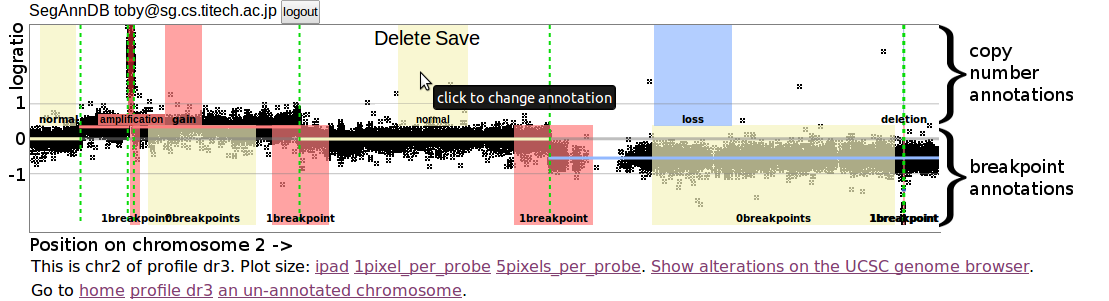
\includegraphics[width=\textwidth]{new-new-annotations}
  \end{center}
  Analyst sees profile $\mathbf x_i$, model $f(\mathbf x_i, \lambda)$,
  and labels $\mathbf \mathbf y_i$ (editable).

  \vskip 0.1in Public SegAnnDB
  server: \url{http://bioviz.rocq.inria.fr/}

\vskip 0.1in
Demo: private server for McGill data sets.
\small
\url{http://ec2-54-201-171-12.us-west-2.compute.amazonaws.com/}

\end{frame}

\begin{frame}
  \frametitle{Supervised, interactive genomic segmentation}
  First step same as supervised, non-interactive model.
  \small
  \begin{displaymath}
  \xymatrix{
    \text{Data $\mathbf x$}
    \ar `[r] [dr] 
    %\ar `r[rr] [drr] 
    %\ar `r[rrr] [drrr] 
    \ar [d]
    & \text{ }
    & \text{ }
    & \text{ }
    \\
    \text{Plot 1} 
    \ar [d]
    & 
    \text{Model $f(\mathbf x, \lambda_1)$} 
    %\ar [r]
    &
    \color{white}{\text{Plot 2} }
    %\ar [d]
    & 
    \color{white}{\text{Model $f(\mathbf x, \lambda_2)$} }
    \\
    \text{Labels $\mathbf y_1$}       
    \ar [d]
    %\ar [rr]
    %\ar [rru]
    &
    &
    \color{white}{\text{Labels $\mathbf y_2$}}
    %\ar [d]
    \\
    \text{Parameter $\lambda_1$} 
    \ar `r[ruu] [ruu]
    & \text{ }
    & 
    \color{white}{\text{Parameter $\lambda_2$}}
    %\ar `r[ruu] [ruu]
  }
  \end{displaymath}
\end{frame}

\begin{frame}
  \frametitle{Supervised, interactive genomic segmentation}
  Plot data, model, and labels.
  \small
  \begin{displaymath}
  \xymatrix{
    \text{Data $\mathbf x$}
    \ar `[r] [dr] 
    \ar `r[rr] [drr] 
    %\ar `r[rrr] [drrr] 
    \ar [d]
    & \text{ }
    & \text{ }
    & \text{ }
    \\
    \text{Plot 1} 
    \ar [d]
    & 
    \text{Model $f(\mathbf x, \lambda_1)$} 
    \ar [r]
    &
    \text{Plot 2} 
    %\ar [d]
    & 
    \color{white}{\text{Model $f(\mathbf x, \lambda_2)$} }
    \\
    \text{Labels $\mathbf y_1$}       
    \ar [d]
    %\ar [rr]
    \ar [rru]
    &
    &
    \color{white}{\text{Labels $\mathbf y_2$}}
    %\ar [d]
    \\
    \text{Parameter $\lambda_1$} 
    \ar `r[ruu] [ruu]
    & \text{ }
    & 
    \color{white}{\text{Parameter $\lambda_2$}}
    %\ar `r[ruu] [ruu]
  }
  \end{displaymath}
\end{frame}

\begin{frame}
  \frametitle{Supervised, interactive genomic segmentation}
  Add/delete labels based on plotted signal/noise.
  \small
  \begin{displaymath}
  \xymatrix{
    \text{Data $\mathbf x$}
    \ar `[r] [dr] 
    \ar `r[rr] [drr] 
    %\ar `r[rrr] [drrr] 
    \ar [d]
    & \text{ }
    & \text{ }
    & \text{ }
    \\
    \text{Plot 1} 
    \ar [d]
    & 
    \text{Model $f(\mathbf x, \lambda_1)$} 
    \ar [r]
    &
    \text{Plot 2} 
    \ar [d]
    & 
    \color{white}{\text{Model $f(\mathbf x, \lambda_2)$} }
    \\
    \text{Labels $\mathbf y_1$}       
    \ar [d]
    \ar [rr]
    \ar [rru]
    &
    &
    \text{Labels $\mathbf y_2$}
    %\ar [d]
    \\
    \text{Parameter $\lambda_1$} 
    \ar `r[ruu] [ruu]
    & \text{ }
    & 
    \color{white}{\text{Parameter $\lambda_2$}}
    %\ar `r[ruu] [ruu]
  }
  \end{displaymath}
\end{frame}

\begin{frame}
  \frametitle{Supervised, interactive genomic segmentation}
  Compute a better parameter.
  \small
  \begin{displaymath}
  \xymatrix{
    \text{Data $\mathbf x$}
    \ar `[r] [dr] 
    \ar `r[rr] [drr] 
    %\ar `r[rrr] [drrr] 
    \ar [d]
    & \text{ }
    & \text{ }
    & \text{ }
    \\
    \text{Plot 1} 
    \ar [d]
    & 
    \text{Model $f(\mathbf x, \lambda_1)$} 
    \ar [r]
    &
    \text{Plot 2} 
    \ar [d]
    & 
    \color{white}{\text{Model $f(\mathbf x, \lambda_2)$} }
    \\
    \text{Labels $\mathbf y_1$}       
    \ar [d]
    \ar [rr]
    \ar [rru]
    &
    &
    \text{Labels $\mathbf y_2$}
    \ar [d]
    \\
    \text{Parameter $\lambda_1$} 
    \ar `r[ruu] [ruu]
    & \text{ }
    & \text{Parameter $\lambda_2$}
    %\ar `r[ruu] [ruu]
  }
  \end{displaymath}
\end{frame}


\begin{frame}
  \frametitle{Supervised, interactive genomic segmentation}
  Compute a better model.
  \small
  \begin{displaymath}
  \xymatrix{
    \text{Data $\mathbf x$}
    \ar `[r] [dr] 
    \ar `r[rr] [drr] 
    \ar `r[rrr] [drrr] 
    \ar [d]
    & \text{ }
    & \text{ }
    & \text{ }
    \\
    \text{Plot 1} 
    \ar [d]
    & 
    \text{Model $f(\mathbf x, \lambda_1)$} 
    \ar [r]
    &
    \text{Plot 2} 
    \ar [d]
    & 
    \text{Model $f(\mathbf x, \lambda_2)$} 
    \\
    \text{Labels $\mathbf y_1$}       
    \ar [d]
    \ar [rr]
    \ar [rru]
    &
    &
    \text{Labels $\mathbf y_2$}
    \ar [d]
    \\
    \text{Parameter $\lambda_1$} 
    \ar `r[ruu] [ruu]
    & \text{ }
    & \text{Parameter $\lambda_2$}
    \ar `r[ruu] [ruu]
  }
  \end{displaymath}
\end{frame}

\begin{frame}
  \frametitle{Test error decreases as profiles are labeled}
  Hocking \textit{et al}. SegAnnDB: interactive web-based genomic
  segmentation. Bioinformatics (2014).
  \begin{center}
    % Created by tikzDevice version 0.7.0 on 2014-02-02 01:44:57
% !TEX encoding = UTF-8 Unicode
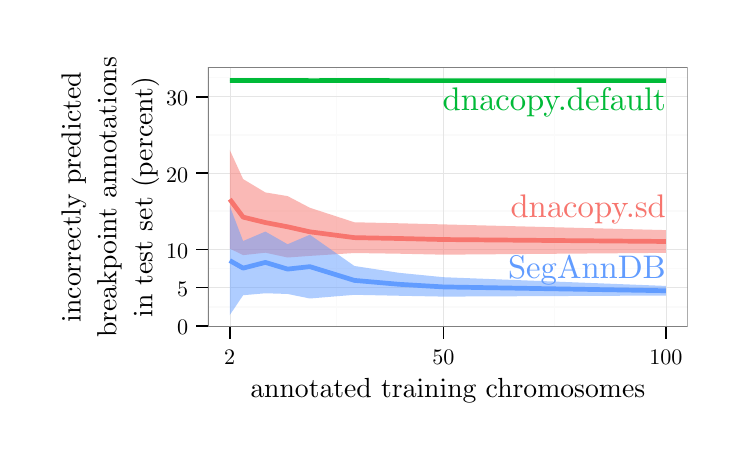
\begin{tikzpicture}[x=1pt,y=1pt]
\definecolor[named]{fillColor}{rgb}{1.00,1.00,1.00}
\path[use as bounding box,fill=fillColor,fill opacity=0.00] (0,0) rectangle (252.94,144.54);
\begin{scope}
\path[clip] (  0.00,  0.00) rectangle (252.94,144.54);
\definecolor[named]{drawColor}{rgb}{1.00,1.00,1.00}
\definecolor[named]{fillColor}{rgb}{1.00,1.00,1.00}

\path[draw=drawColor,line width= 0.6pt,line join=round,line cap=round,fill=fillColor] (  0.00,  0.00) rectangle (252.94,144.54);
\end{scope}
\begin{scope}
\path[clip] ( 65.15, 36.44) rectangle (238.49,130.09);
\definecolor[named]{fillColor}{rgb}{1.00,1.00,1.00}

\path[fill=fillColor] ( 65.15, 36.44) rectangle (238.49,130.09);
\definecolor[named]{drawColor}{rgb}{0.98,0.98,0.98}

\path[draw=drawColor,line width= 0.6pt,line join=round] ( 65.15, 43.70) --
	(238.49, 43.70);

\path[draw=drawColor,line width= 0.6pt,line join=round] ( 65.15, 57.50) --
	(238.49, 57.50);

\path[draw=drawColor,line width= 0.6pt,line join=round] ( 65.15, 78.19) --
	(238.49, 78.19);

\path[draw=drawColor,line width= 0.6pt,line join=round] ( 65.15,105.79) --
	(238.49,105.79);

\path[draw=drawColor,line width= 0.6pt,line join=round] ( 65.15,126.49) --
	(238.49,126.49);

\path[draw=drawColor,line width= 0.6pt,line join=round] (111.62, 36.44) --
	(111.62,130.09);

\path[draw=drawColor,line width= 0.6pt,line join=round] (190.41, 36.44) --
	(190.41,130.09);
\definecolor[named]{drawColor}{rgb}{0.90,0.90,0.90}

\path[draw=drawColor,line width= 0.2pt,line join=round] ( 65.15, 36.80) --
	(238.49, 36.80);

\path[draw=drawColor,line width= 0.2pt,line join=round] ( 65.15, 50.60) --
	(238.49, 50.60);

\path[draw=drawColor,line width= 0.2pt,line join=round] ( 65.15, 64.40) --
	(238.49, 64.40);

\path[draw=drawColor,line width= 0.2pt,line join=round] ( 65.15, 91.99) --
	(238.49, 91.99);

\path[draw=drawColor,line width= 0.2pt,line join=round] ( 65.15,119.59) --
	(238.49,119.59);

\path[draw=drawColor,line width= 0.2pt,line join=round] ( 73.03, 36.44) --
	( 73.03,130.09);

\path[draw=drawColor,line width= 0.2pt,line join=round] (150.21, 36.44) --
	(150.21,130.09);

\path[draw=drawColor,line width= 0.2pt,line join=round] (230.61, 36.44) --
	(230.61,130.09);
\definecolor[named]{drawColor}{rgb}{0.97,0.46,0.43}

\path[draw=drawColor,line width= 1.7pt,line join=round] ( 73.03, 82.53) --
	( 77.85, 76.08) --
	( 85.89, 74.12) --
	( 93.93, 72.58) --
	(101.97, 70.77) --
	(118.05, 68.67) --
	(134.13, 68.36) --
	(150.21, 67.98) --
	(230.61, 67.28);
\definecolor[named]{drawColor}{rgb}{0.00,0.73,0.22}

\path[draw=drawColor,line width= 1.7pt,line join=round] ( 73.03,125.46) --
	( 77.85,125.46) --
	( 85.89,125.45) --
	( 93.93,125.44) --
	(101.97,125.41) --
	(118.05,125.42) --
	(134.13,125.41) --
	(150.21,125.40) --
	(230.61,125.40);
\definecolor[named]{drawColor}{rgb}{0.38,0.61,1.00}

\path[draw=drawColor,line width= 1.7pt,line join=round] ( 73.03, 60.38) --
	( 77.85, 57.65) --
	( 85.89, 59.72) --
	( 93.93, 57.30) --
	(101.97, 58.19) --
	(118.05, 53.22) --
	(134.13, 51.81) --
	(150.21, 50.86) --
	(230.61, 49.48);
\definecolor[named]{fillColor}{rgb}{0.97,0.46,0.43}

\path[fill=fillColor,fill opacity=0.50] ( 73.03,100.34) --
	( 77.85, 89.82) --
	( 85.89, 85.00) --
	( 93.93, 83.67) --
	(101.97, 79.46) --
	(118.05, 74.22) --
	(134.13, 73.86) --
	(150.21, 73.45) --
	(230.61, 71.39) --
	(230.61, 63.17) --
	(150.21, 62.51) --
	(134.13, 62.86) --
	(118.05, 63.11) --
	(101.97, 62.07) --
	( 93.93, 61.49) --
	( 85.89, 63.23) --
	( 77.85, 62.34) --
	( 73.03, 64.73) --
	cycle;
\definecolor[named]{fillColor}{rgb}{0.00,0.73,0.22}

\path[fill=fillColor,fill opacity=0.50] ( 73.03,125.51) --
	( 77.85,125.55) --
	( 85.89,125.58) --
	( 93.93,125.60) --
	(101.97,125.58) --
	(118.05,125.64) --
	(134.13,125.67) --
	(150.21,125.70) --
	(230.61,125.83) --
	(230.61,124.96) --
	(150.21,125.10) --
	(134.13,125.15) --
	(118.05,125.20) --
	(101.97,125.25) --
	( 93.93,125.28) --
	( 85.89,125.31) --
	( 77.85,125.37) --
	( 73.03,125.41) --
	cycle;
\definecolor[named]{fillColor}{rgb}{0.38,0.61,1.00}

\path[fill=fillColor,fill opacity=0.50] ( 73.03, 80.06) --
	( 77.85, 67.44) --
	( 85.89, 70.86) --
	( 93.93, 66.28) --
	(101.97, 69.71) --
	(118.05, 58.43) --
	(134.13, 55.96) --
	(150.21, 54.37) --
	(230.61, 51.22) --
	(230.61, 47.75) --
	(150.21, 47.36) --
	(134.13, 47.67) --
	(118.05, 48.01) --
	(101.97, 46.68) --
	( 93.93, 48.32) --
	( 85.89, 48.57) --
	( 77.85, 47.86) --
	( 73.03, 40.70) --
	cycle;
\definecolor[named]{drawColor}{rgb}{0.00,0.73,0.22}

\node[text=drawColor,anchor=base east,inner sep=0pt, outer sep=0pt, scale=  1.18] at (230.61,114.71) {dnacopy.default};
\definecolor[named]{drawColor}{rgb}{0.97,0.46,0.43}

\node[text=drawColor,anchor=base east,inner sep=0pt, outer sep=0pt, scale=  1.18] at (230.61, 76.07) {dnacopy.sd};
\definecolor[named]{drawColor}{rgb}{0.38,0.61,1.00}

\node[text=drawColor,anchor=base east,inner sep=0pt, outer sep=0pt, scale=  1.18] at (230.61, 54.00) {SegAnnDB};
\definecolor[named]{drawColor}{rgb}{0.50,0.50,0.50}

\path[draw=drawColor,line width= 0.6pt,line join=round,line cap=round] ( 65.15, 36.44) rectangle (238.49,130.09);
\end{scope}
\begin{scope}
\path[clip] (  0.00,  0.00) rectangle (252.94,144.54);
\definecolor[named]{drawColor}{rgb}{0.00,0.00,0.00}

\node[text=drawColor,anchor=base east,inner sep=0pt, outer sep=0pt, scale=  0.80] at ( 58.04, 33.50) {0};

\node[text=drawColor,anchor=base east,inner sep=0pt, outer sep=0pt, scale=  0.80] at ( 58.04, 47.29) {5};

\node[text=drawColor,anchor=base east,inner sep=0pt, outer sep=0pt, scale=  0.80] at ( 58.04, 61.09) {10};

\node[text=drawColor,anchor=base east,inner sep=0pt, outer sep=0pt, scale=  0.80] at ( 58.04, 88.69) {20};

\node[text=drawColor,anchor=base east,inner sep=0pt, outer sep=0pt, scale=  0.80] at ( 58.04,116.28) {30};
\end{scope}
\begin{scope}
\path[clip] (  0.00,  0.00) rectangle (252.94,144.54);
\definecolor[named]{drawColor}{rgb}{0.00,0.00,0.00}

\path[draw=drawColor,line width= 0.6pt,line join=round] ( 60.88, 36.80) --
	( 65.15, 36.80);

\path[draw=drawColor,line width= 0.6pt,line join=round] ( 60.88, 50.60) --
	( 65.15, 50.60);

\path[draw=drawColor,line width= 0.6pt,line join=round] ( 60.88, 64.40) --
	( 65.15, 64.40);

\path[draw=drawColor,line width= 0.6pt,line join=round] ( 60.88, 91.99) --
	( 65.15, 91.99);

\path[draw=drawColor,line width= 0.6pt,line join=round] ( 60.88,119.59) --
	( 65.15,119.59);
\end{scope}
\begin{scope}
\path[clip] (  0.00,  0.00) rectangle (252.94,144.54);
\definecolor[named]{drawColor}{rgb}{0.00,0.00,0.00}

\path[draw=drawColor,line width= 0.6pt,line join=round] ( 73.03, 32.18) --
	( 73.03, 36.44);

\path[draw=drawColor,line width= 0.6pt,line join=round] (150.21, 32.18) --
	(150.21, 36.44);

\path[draw=drawColor,line width= 0.6pt,line join=round] (230.61, 32.18) --
	(230.61, 36.44);
\end{scope}
\begin{scope}
\path[clip] (  0.00,  0.00) rectangle (252.94,144.54);
\definecolor[named]{drawColor}{rgb}{0.00,0.00,0.00}

\node[text=drawColor,anchor=base,inner sep=0pt, outer sep=0pt, scale=  0.80] at ( 73.03, 22.72) {2};

\node[text=drawColor,anchor=base,inner sep=0pt, outer sep=0pt, scale=  0.80] at (150.21, 22.72) {50};

\node[text=drawColor,anchor=base,inner sep=0pt, outer sep=0pt, scale=  0.80] at (230.61, 22.72) {100};
\end{scope}
\begin{scope}
\path[clip] (  0.00,  0.00) rectangle (252.94,144.54);
\definecolor[named]{drawColor}{rgb}{0.00,0.00,0.00}

\node[text=drawColor,anchor=base,inner sep=0pt, outer sep=0pt, scale=  1.00] at (151.82, 10.84) {annotated training chromosomes};
\end{scope}
\begin{scope}
\path[clip] (  0.00,  0.00) rectangle (252.94,144.54);
\definecolor[named]{drawColor}{rgb}{0.00,0.00,0.00}

\node[text=drawColor,rotate= 90.00,anchor=base,inner sep=0pt, outer sep=0pt, scale=  1.00] at ( 19.11, 83.26) {incorrectly predicted};

\node[text=drawColor,rotate= 90.00,anchor=base,inner sep=0pt, outer sep=0pt, scale=  1.00] at ( 32.07, 83.26) {breakpoint annotations};

\node[text=drawColor,rotate= 90.00,anchor=base,inner sep=0pt, outer sep=0pt, scale=  1.00] at ( 45.03, 83.26) {in test set (percent)};
\end{scope}
\end{tikzpicture}

  \end{center}
\end{frame}

\begin{frame}
  \frametitle{Summary of contributions to
    DNA copy number analysis}
  \begin{center}
  \begin{tabular}{c|c|c}
    Evaluation: & qualitative &  quantitative \\
    Input: profile $\mathbf x$ + & parameters $\lambda$ & labels $\mathbf y$ \\
        & \textbf{unsupervised} & \textbf{supervised}\\
    \hline
    \textbf{non-interactive}
    & plot $\mathbf x$ & plot $\mathbf x, \mathbf y$\\
    fit one model
    & default parameters $\lambda$ & trained parameters $\lambda$ \\
    & e.g. DNAcopy & BMC'13, ICML'13\\
    \hline
    \textbf{interactive}
    & plot $\mathbf x, f(\mathbf x, \lambda)$ 
    & plot $\mathbf x, \mathbf y, f(\mathbf x, \lambda)$\\
    plot, update model 
    & manually tuned $\lambda$ & iterative $\lambda$ training\\
    & e.g. CGHweb  & Bioinfo'14
  \end{tabular}
  \end{center}
  \begin{description}
  % \item[2004-now] dozens of \textbf{unsupervised} models that can be
  %   \textbf{tweaked} e.g. GLAD, DNAcopy, fused lasso, cghseg, PELT.
  % \item[2009-2010] \textbf{No model $f$}! Breakpoint labels recorded
  %   by typing 0/1 in Excel spreadsheets (Janoueix-Lerosey,
  %   Schleiermacher, \textit{et al.} J Clinical Oncology).
  \item[BMC'13] \textbf{Non-interactive, supervised, single-parameter}.
    Learning smoothing models of copy number profiles... 
    BMC Bioinformatics, Hocking \textit{et al}.
  \item[ICML'13] \textbf{Non-interactive, supervised,
      multi-parameter}.  
    Learning sparse penalties... Hocking \textit{et al}.
  \item[Bioinfo'14] \textbf{Interactive, supervised, multi-parameter}.
    SegAnnDB..., Bioinformatics, Hocking \textit{et al}.
  \end{description}
\end{frame}

\section{Supervised ChIP-seq peak detection}

\begin{frame}
  \frametitle{A brief history of supervised ChIP-seq peak detection}
  \begin{description}
  \item[2011] Rye et al. Manually labeled sites and visual peaks for 3
    transcription factors.\\
    \textbf{Model evaluation.}
  \item[2014] Hocking et al. arXiv:1409.6209. Manually labeled visual
    peaks for 2 histone marks, 4 different annotators.
    \\
    \textbf{Single-parameter model training and evaluation.}\\
    Hocking et al. PeakSeg. NIPS Computational Biology workshop.\\
    \textbf{fo}
  \item[2015] 
  \end{description}
\end{frame}

\begin{frame}
  \frametitle{Two annotators agree on the same profile}
  
  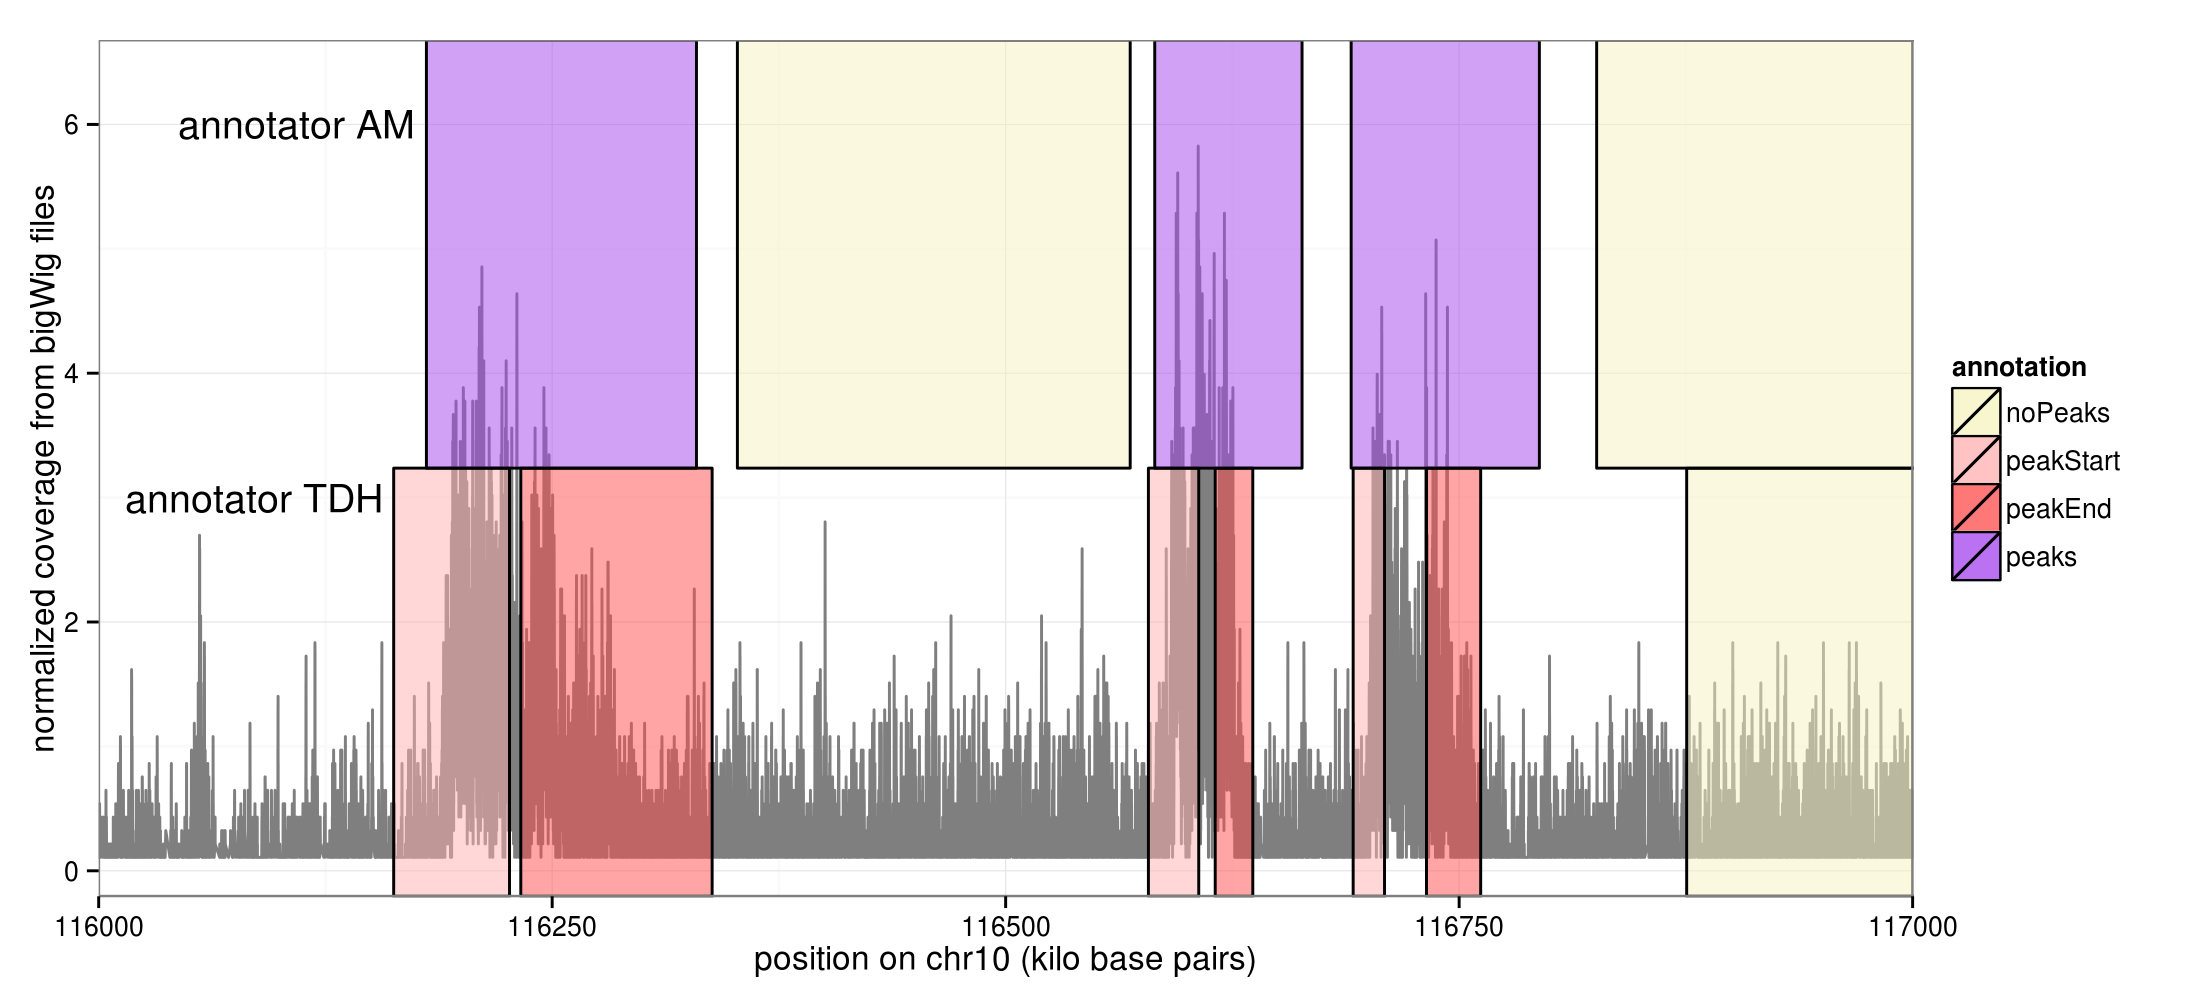
\includegraphics[width=\textwidth]{figure-several-annotators}
\end{frame}

\begin{frame} 
  \frametitle{Advantages of supervised learning}
  Creating data sets $\mathbf x$ with labels $\mathbf y$ is important for
  \begin{description}
  \item[short-term] quantitative evaluation, more convincing papers.
  \item[long-term] cross-discipline collaboration!
    \begin{description}
    \item[statisticians/modelers] get better evaluation
    metrics.
    \item[biologists/annotators] get
    better models.
    \end{description}
  \end{description}

  Can we make labels/supervised approaches for...
  \begin{description}
  \item[segmentation] breakpoint/copy number regions (this work).
  \item[clustering] pairs that should join (or not)?
  \item[regression] variables/genes that are important (or not)?
  \item[diff expression] genes that are up/down (or not)?
  \end{description}
  Write me at \texttt{toby.hocking@mail.mcgill.ca} to collaborate!
\end{frame}

\begin{frame}
  \frametitle{Thank you!}
  Supplementary slides appear after this one.

  \vskip 1cm

  Source code for slides online!\\
  \small
  \url{https://github.com/tdhock/supervised-interactive-slides}
\end{frame}

\end{document}
